\documentclass[11pt]{article}
\usepackage[textwidth=18.0cm, textheight=23.0cm, top=2.0cm]{geometry}
\usepackage{pst-all}
\usepackage{amssymb}
\usepackage{tikz}
\usepackage{underscore}\begin{document}
\pagestyle{empty}


ClassName: \underline{\textbf{Class_08.2bp-10}}
\par
BinSize: \underline{\textbf{100 × 100}}
\par
ReduceSize: \underline{\textbf{100 × 100}}
\par
TypeNum: \underline{\textbf{39}}
\par
Num: \underline{\textbf{40}}
\par
OutS: \underline{\textbf{120000}}
\par
InS: \underline{\textbf{95261}}
\par
Rate: \underline{\textbf{0.794}}
\par
UB: \underline{\textbf{12}}
\par
LB0: \underline{\textbf{11}}
\par
LB: \underline{\textbf{12}}
\par
LBWithCut: \underline{\textbf{12}}
\par
NodeCut: \underline{\textbf{0}}
\par
ExtendedNodeCnt: \underline{\textbf{1}}
\par
GenNodeCnt: \underline{\textbf{1}}
\par
PrimalNode: \underline{\textbf{0}}
\par
ColumnCount: \underline{\textbf{109}}
\par
TotalCutCount: \underline{\textbf{0}}
\par
RootCutCount: \underline{\textbf{0}}
\par
LPSolverCnt: \underline{\textbf{98}}
\par
PricingSolverCnt: \underline{\textbf{98}}
\par
BranchAndBoundNum: \underline{\textbf{1}}
\par
isOpt: \underline{\textbf{true}}
\par
TimeOnPrimal: \underline{\textbf{0.000 s}}
\par
TimeOnPricing: \underline{\textbf{6.733 s}}
\par
TimeOnRmp: \underline{\textbf{0.157 s}}
\par
TotalTime: \underline{\textbf{6.937 s}}
\par
\newpage


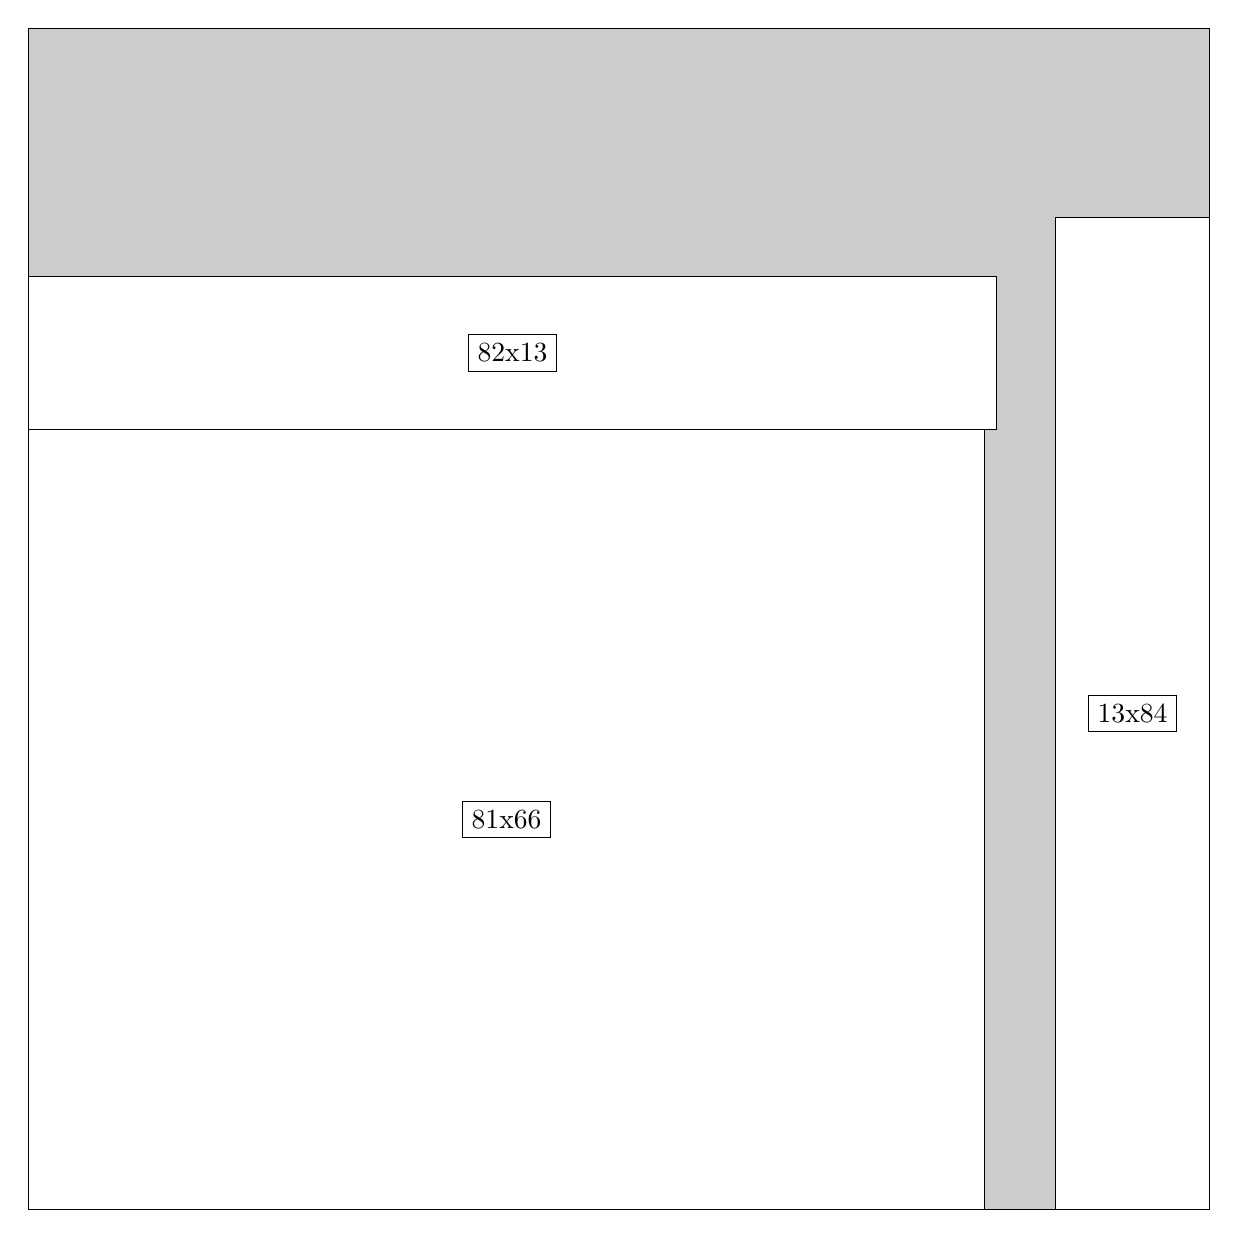
\begin{tikzpicture}[shorten >=1pt,scale=1.0,every node/.style={scale=1.0},->]
\tikzstyle{vertex}=[circle,fill=black!25,minimum size=14pt,inner sep=0pt]
\filldraw[fill=gray!40!white, draw=black] (0,0) rectangle (15.0,15.0);
\foreach \name/\x/\y/\w/\h in {81x66/0.0/0.0/12.15/9.9,13x84/13.049999999999999/0.0/1.95/12.6,82x13/0.0/9.9/12.299999999999999/1.95}
\filldraw[fill=white!40!white, draw=black] (\x,\y) rectangle node[draw] (\name) {\name} ++(\w,\h);
\end{tikzpicture}


w =81 , h =66 , x =0 , y =0 , v =5346
\par
w =13 , h =84 , x =87 , y =0 , v =1092
\par
w =82 , h =13 , x =0 , y =66 , v =1066
\par
\newpage


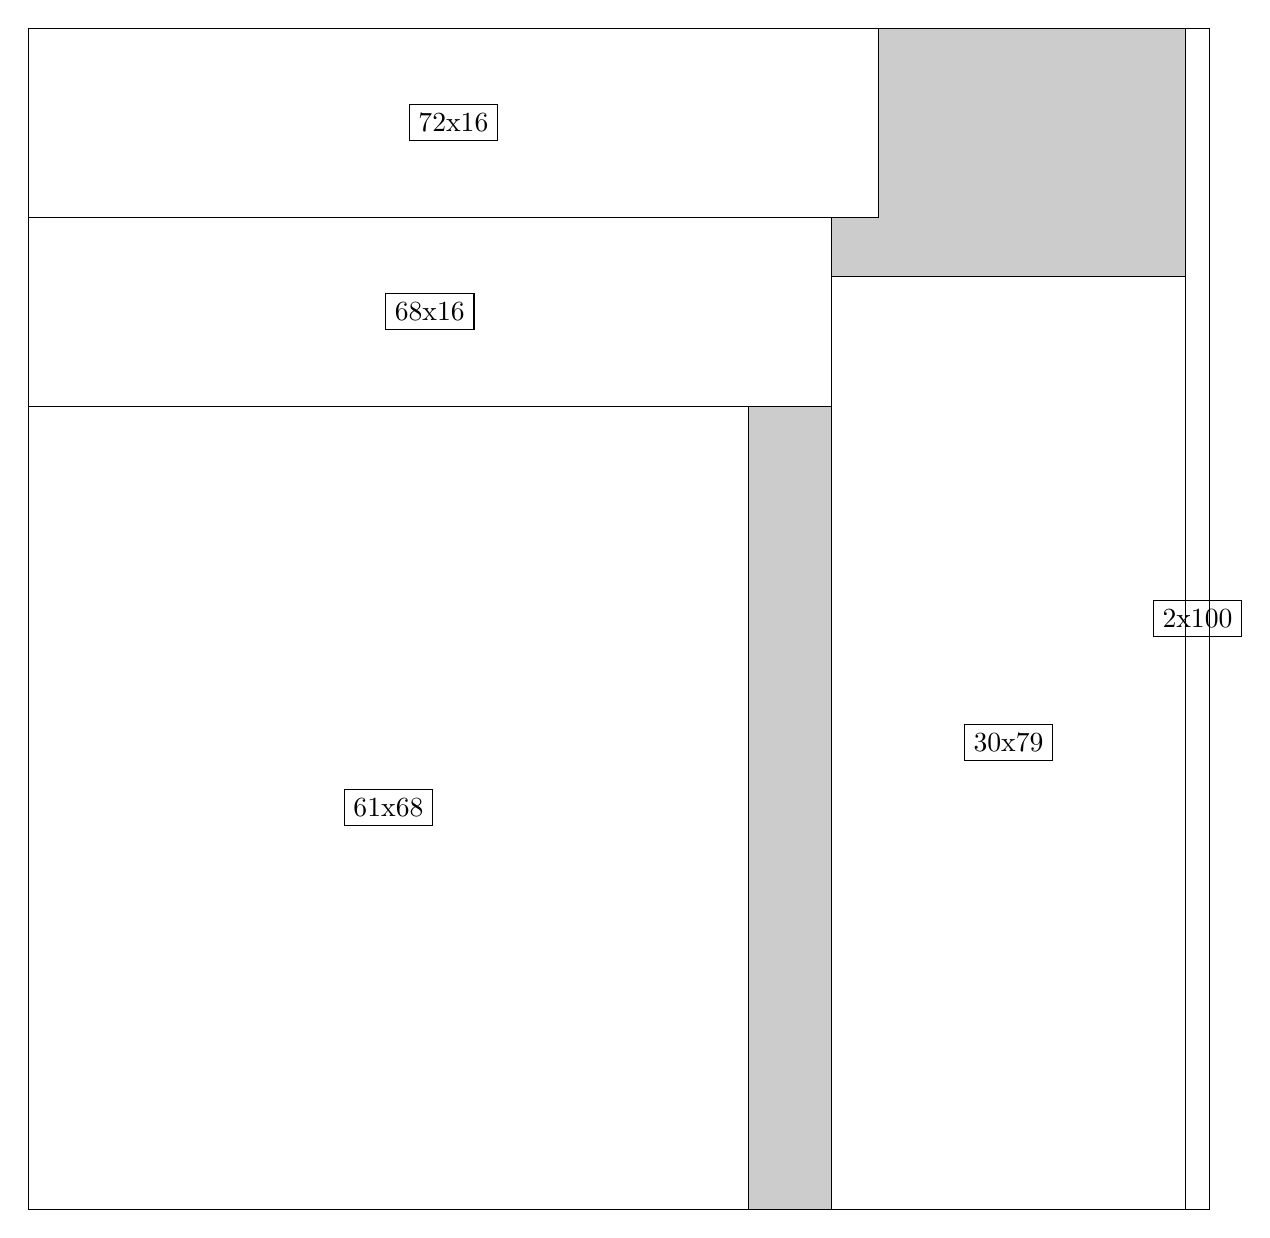
\begin{tikzpicture}[shorten >=1pt,scale=1.0,every node/.style={scale=1.0},->]
\tikzstyle{vertex}=[circle,fill=black!25,minimum size=14pt,inner sep=0pt]
\filldraw[fill=gray!40!white, draw=black] (0,0) rectangle (15.0,15.0);
\foreach \name/\x/\y/\w/\h in {61x68/0.0/0.0/9.15/10.2,30x79/10.2/0.0/4.5/11.85,72x16/0.0/12.6/10.799999999999999/2.4,68x16/0.0/10.2/10.2/2.4,2x100/14.7/0.0/0.3/15.0}
\filldraw[fill=white!40!white, draw=black] (\x,\y) rectangle node[draw] (\name) {\name} ++(\w,\h);
\end{tikzpicture}


w =61 , h =68 , x =0 , y =0 , v =4148
\par
w =30 , h =79 , x =68 , y =0 , v =2370
\par
w =72 , h =16 , x =0 , y =84 , v =1152
\par
w =68 , h =16 , x =0 , y =68 , v =1088
\par
w =2 , h =100 , x =98 , y =0 , v =200
\par
\newpage


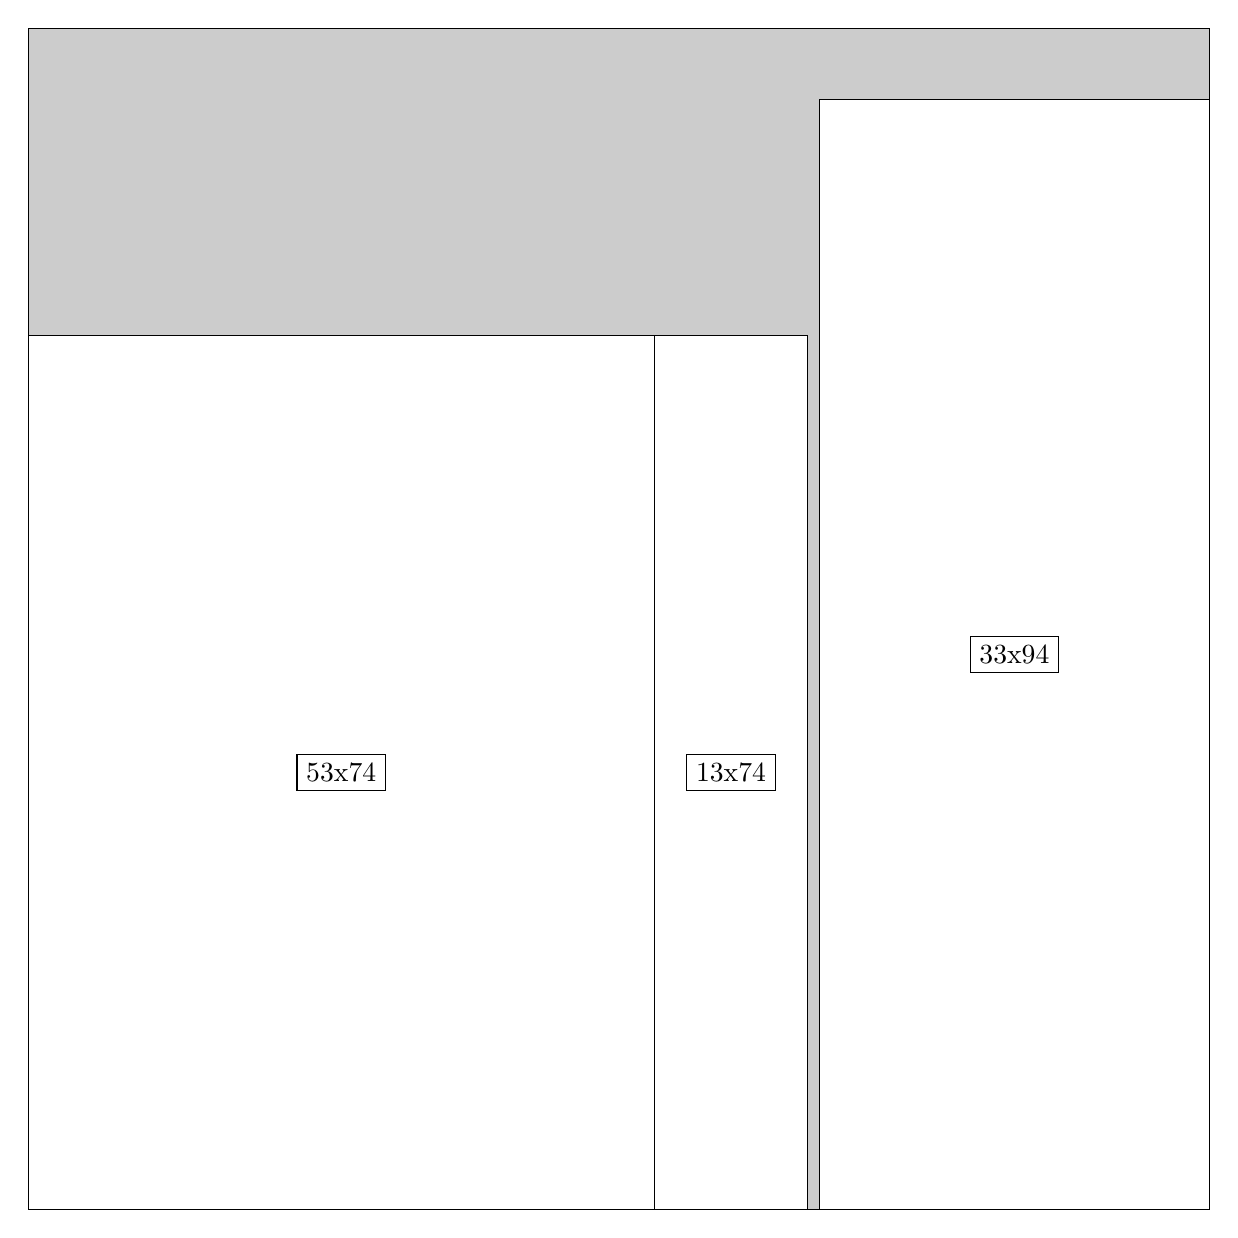
\begin{tikzpicture}[shorten >=1pt,scale=1.0,every node/.style={scale=1.0},->]
\tikzstyle{vertex}=[circle,fill=black!25,minimum size=14pt,inner sep=0pt]
\filldraw[fill=gray!40!white, draw=black] (0,0) rectangle (15.0,15.0);
\foreach \name/\x/\y/\w/\h in {53x74/0.0/0.0/7.949999999999999/11.1,33x94/10.049999999999999/0.0/4.95/14.1,13x74/7.949999999999999/0.0/1.95/11.1}
\filldraw[fill=white!40!white, draw=black] (\x,\y) rectangle node[draw] (\name) {\name} ++(\w,\h);
\end{tikzpicture}


w =53 , h =74 , x =0 , y =0 , v =3922
\par
w =33 , h =94 , x =67 , y =0 , v =3102
\par
w =13 , h =74 , x =53 , y =0 , v =962
\par
\newpage


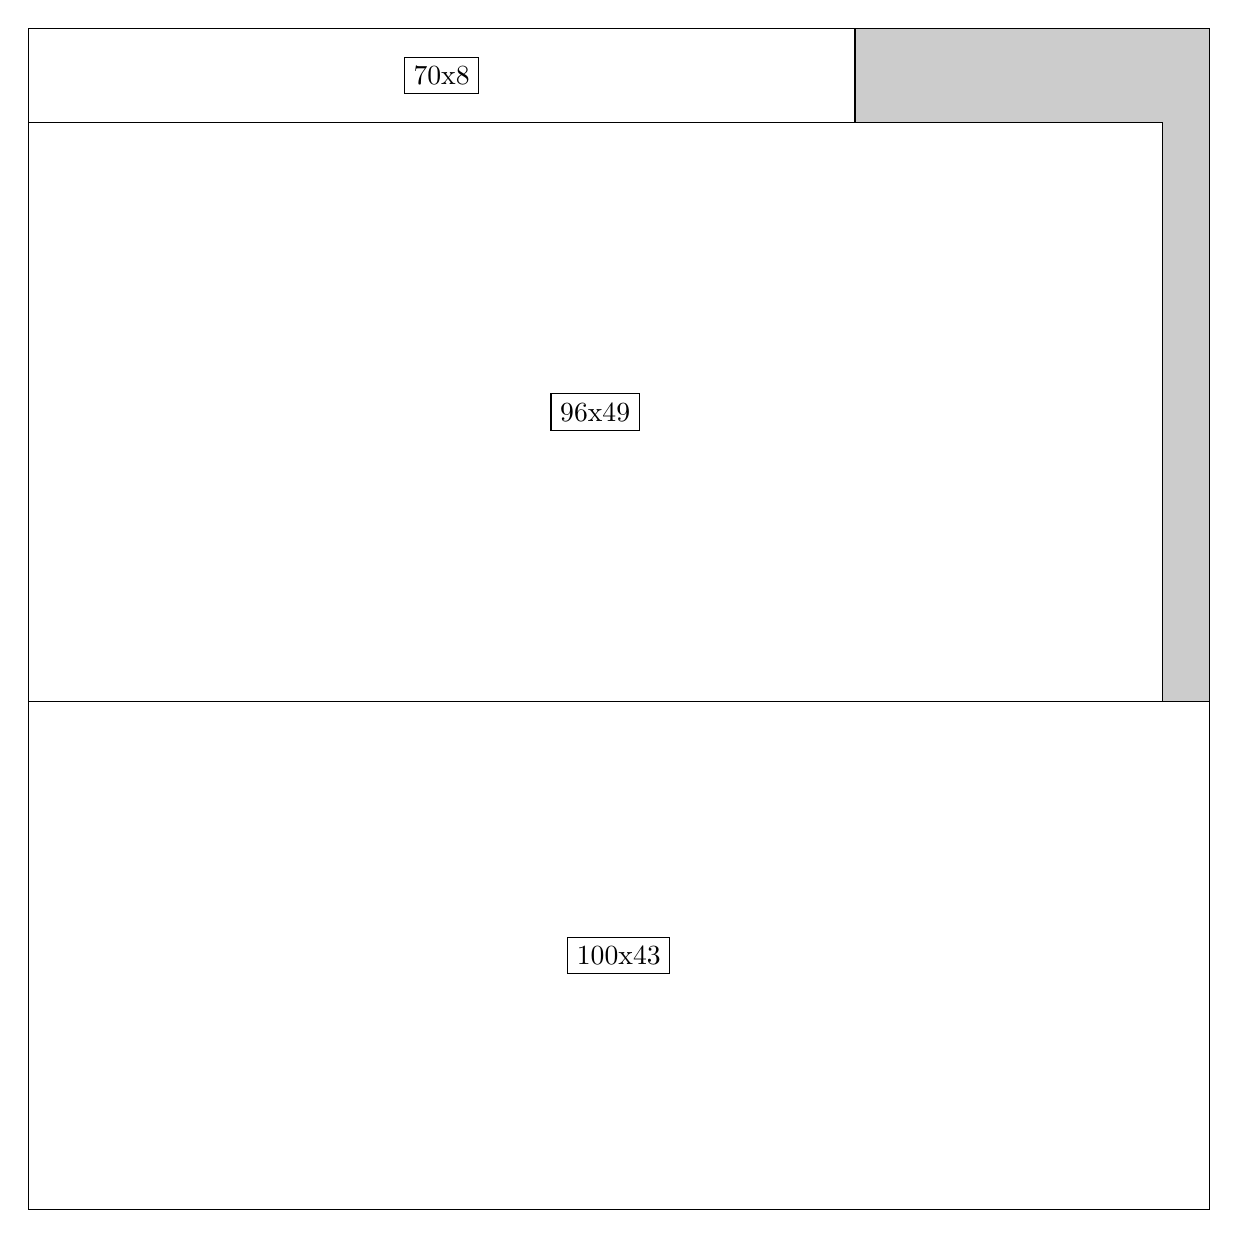
\begin{tikzpicture}[shorten >=1pt,scale=1.0,every node/.style={scale=1.0},->]
\tikzstyle{vertex}=[circle,fill=black!25,minimum size=14pt,inner sep=0pt]
\filldraw[fill=gray!40!white, draw=black] (0,0) rectangle (15.0,15.0);
\foreach \name/\x/\y/\w/\h in {96x49/0.0/6.45/14.399999999999999/7.35,100x43/0.0/0.0/15.0/6.45,70x8/0.0/13.799999999999999/10.5/1.2}
\filldraw[fill=white!40!white, draw=black] (\x,\y) rectangle node[draw] (\name) {\name} ++(\w,\h);
\end{tikzpicture}


w =96 , h =49 , x =0 , y =43 , v =4704
\par
w =100 , h =43 , x =0 , y =0 , v =4300
\par
w =70 , h =8 , x =0 , y =92 , v =560
\par
\newpage


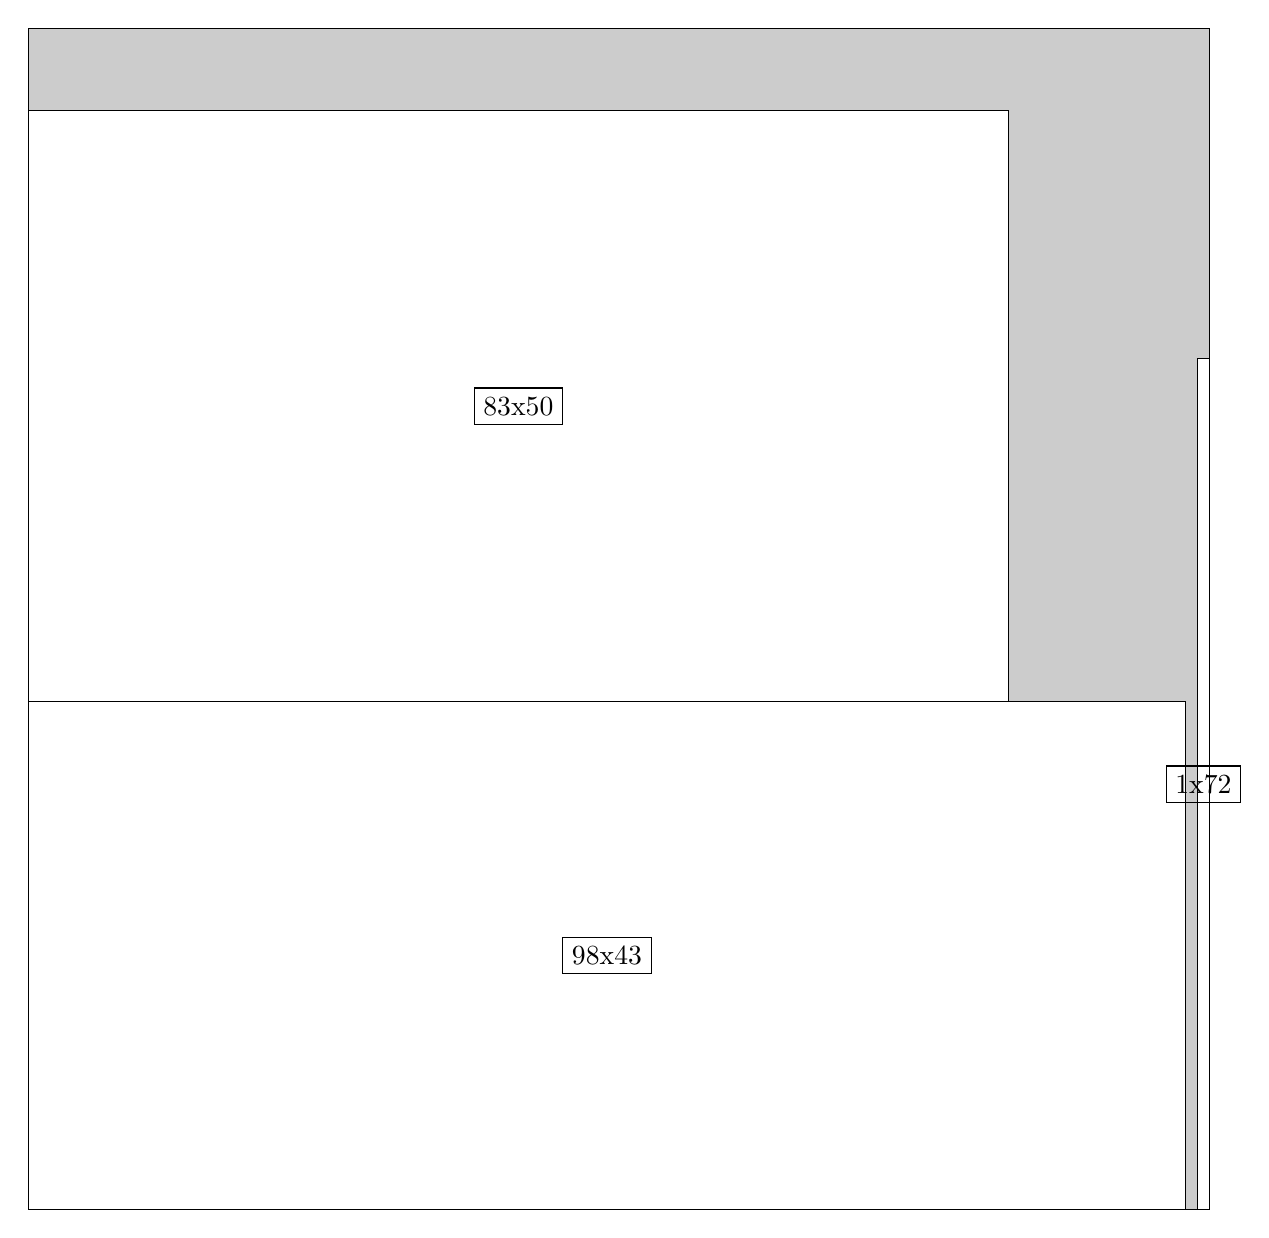
\begin{tikzpicture}[shorten >=1pt,scale=1.0,every node/.style={scale=1.0},->]
\tikzstyle{vertex}=[circle,fill=black!25,minimum size=14pt,inner sep=0pt]
\filldraw[fill=gray!40!white, draw=black] (0,0) rectangle (15.0,15.0);
\foreach \name/\x/\y/\w/\h in {98x43/0.0/0.0/14.7/6.45,83x50/0.0/6.45/12.45/7.5,1x72/14.85/0.0/0.15/10.799999999999999}
\filldraw[fill=white!40!white, draw=black] (\x,\y) rectangle node[draw] (\name) {\name} ++(\w,\h);
\end{tikzpicture}


w =98 , h =43 , x =0 , y =0 , v =4214
\par
w =83 , h =50 , x =0 , y =43 , v =4150
\par
w =1 , h =72 , x =99 , y =0 , v =72
\par
\newpage


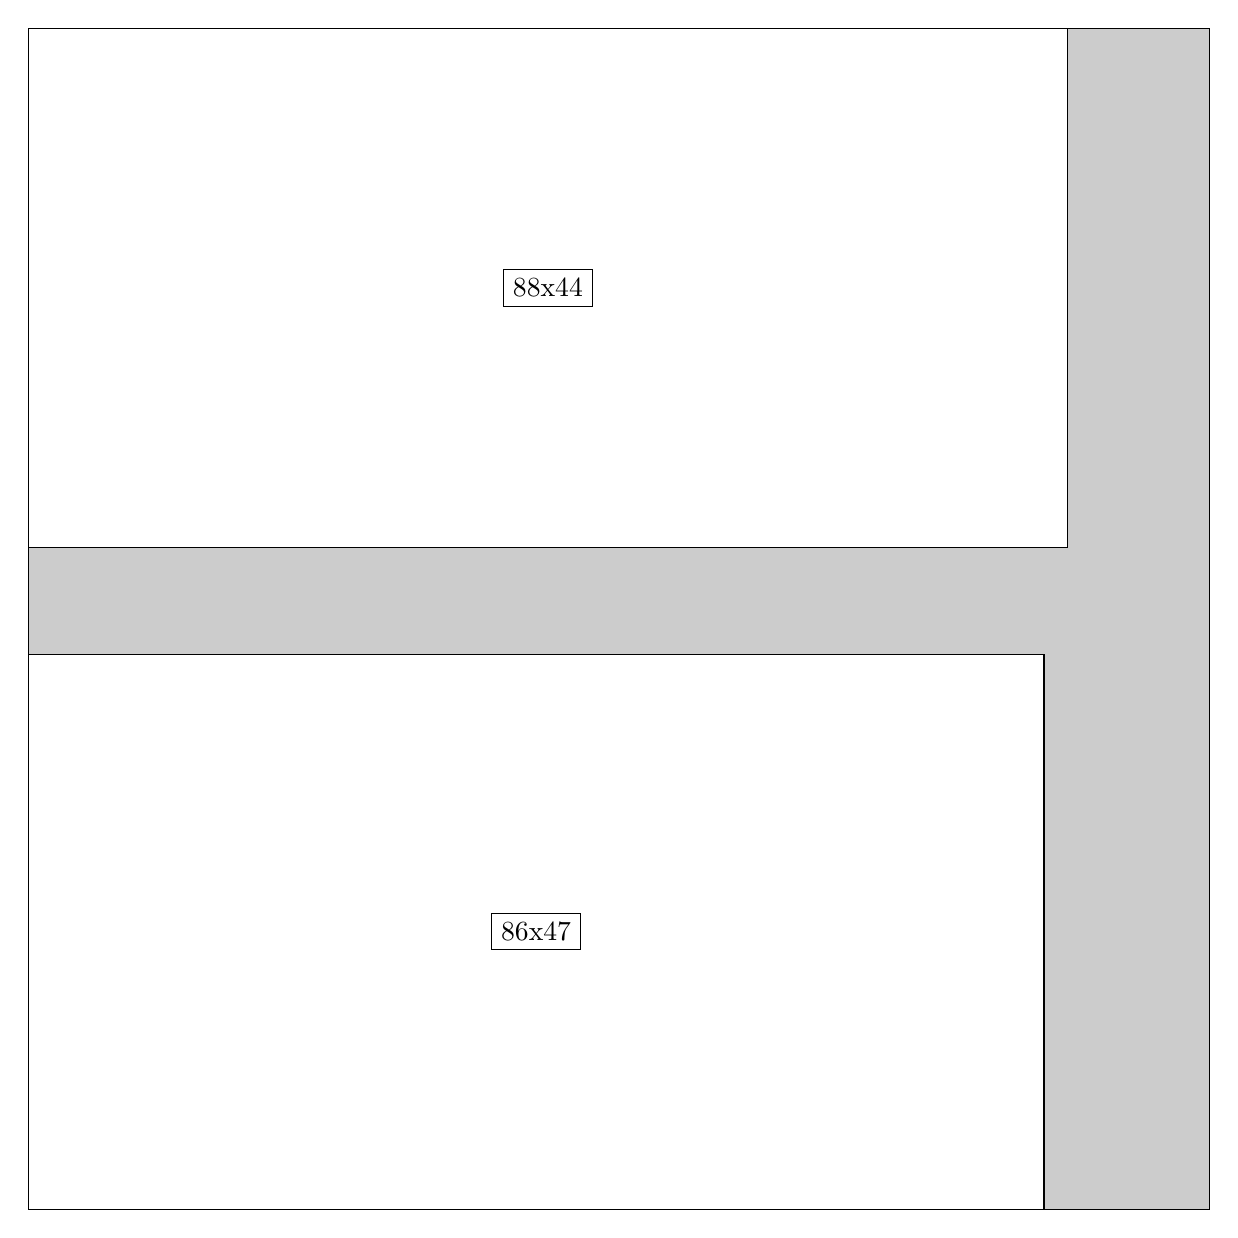
\begin{tikzpicture}[shorten >=1pt,scale=1.0,every node/.style={scale=1.0},->]
\tikzstyle{vertex}=[circle,fill=black!25,minimum size=14pt,inner sep=0pt]
\filldraw[fill=gray!40!white, draw=black] (0,0) rectangle (15.0,15.0);
\foreach \name/\x/\y/\w/\h in {86x47/0.0/0.0/12.9/7.05,88x44/0.0/8.4/13.2/6.6}
\filldraw[fill=white!40!white, draw=black] (\x,\y) rectangle node[draw] (\name) {\name} ++(\w,\h);
\end{tikzpicture}


w =86 , h =47 , x =0 , y =0 , v =4042
\par
w =88 , h =44 , x =0 , y =56 , v =3872
\par
\newpage


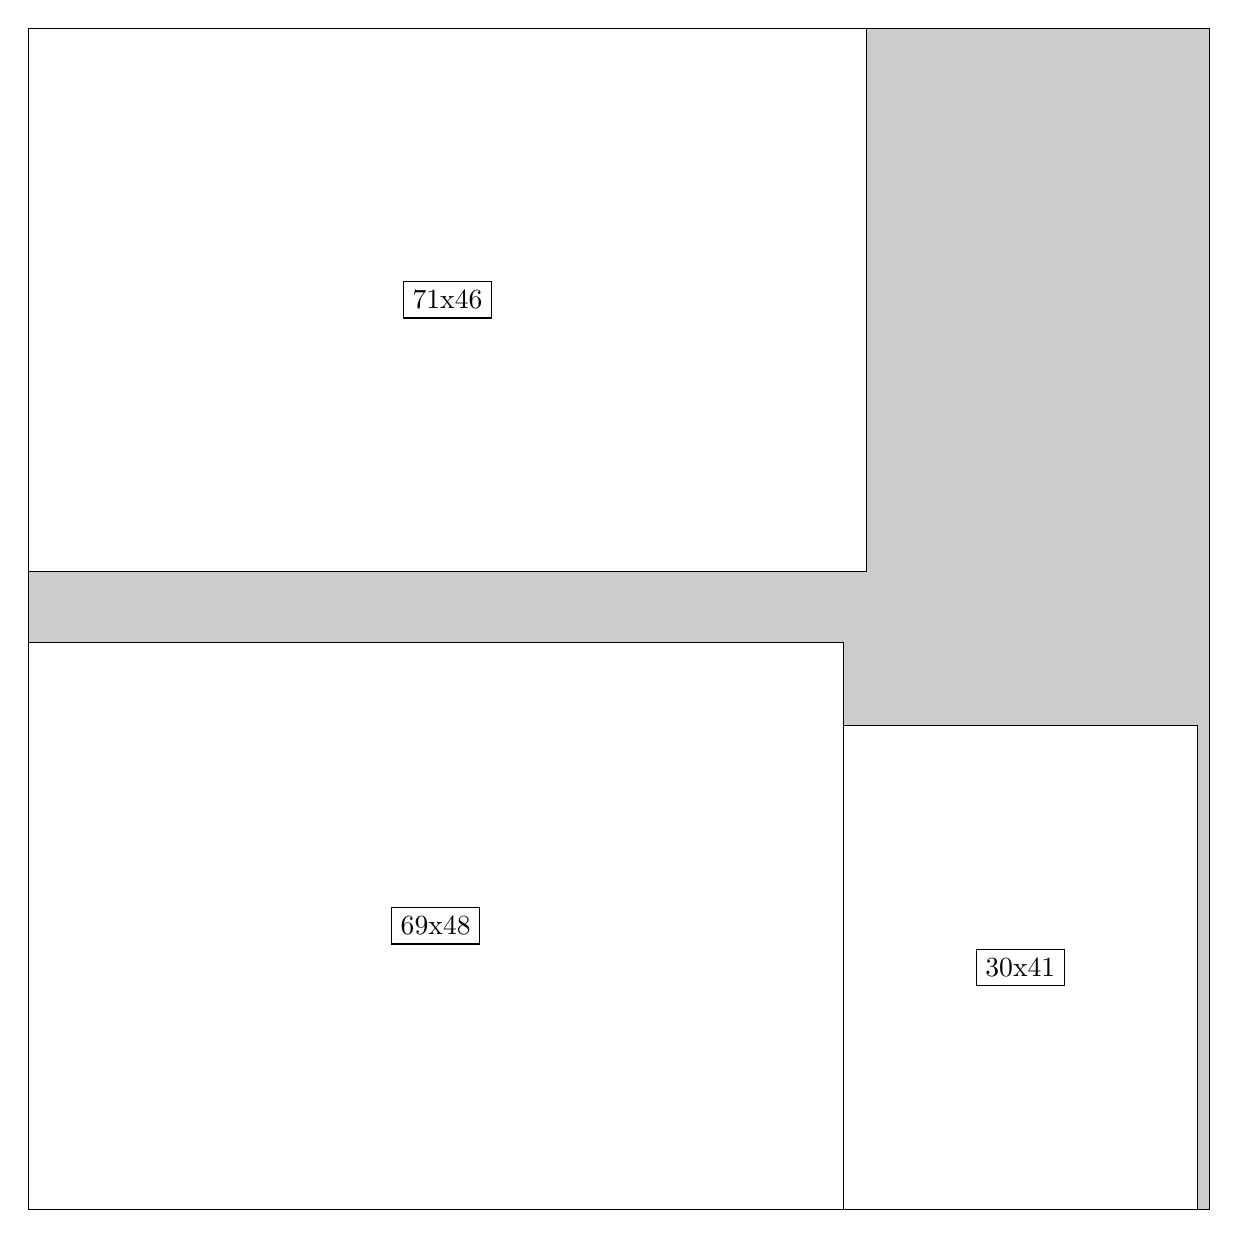
\begin{tikzpicture}[shorten >=1pt,scale=1.0,every node/.style={scale=1.0},->]
\tikzstyle{vertex}=[circle,fill=black!25,minimum size=14pt,inner sep=0pt]
\filldraw[fill=gray!40!white, draw=black] (0,0) rectangle (15.0,15.0);
\foreach \name/\x/\y/\w/\h in {69x48/0.0/0.0/10.35/7.199999999999999,71x46/0.0/8.1/10.65/6.8999999999999995,30x41/10.35/0.0/4.5/6.1499999999999995}
\filldraw[fill=white!40!white, draw=black] (\x,\y) rectangle node[draw] (\name) {\name} ++(\w,\h);
\end{tikzpicture}


w =69 , h =48 , x =0 , y =0 , v =3312
\par
w =71 , h =46 , x =0 , y =54 , v =3266
\par
w =30 , h =41 , x =69 , y =0 , v =1230
\par
\newpage


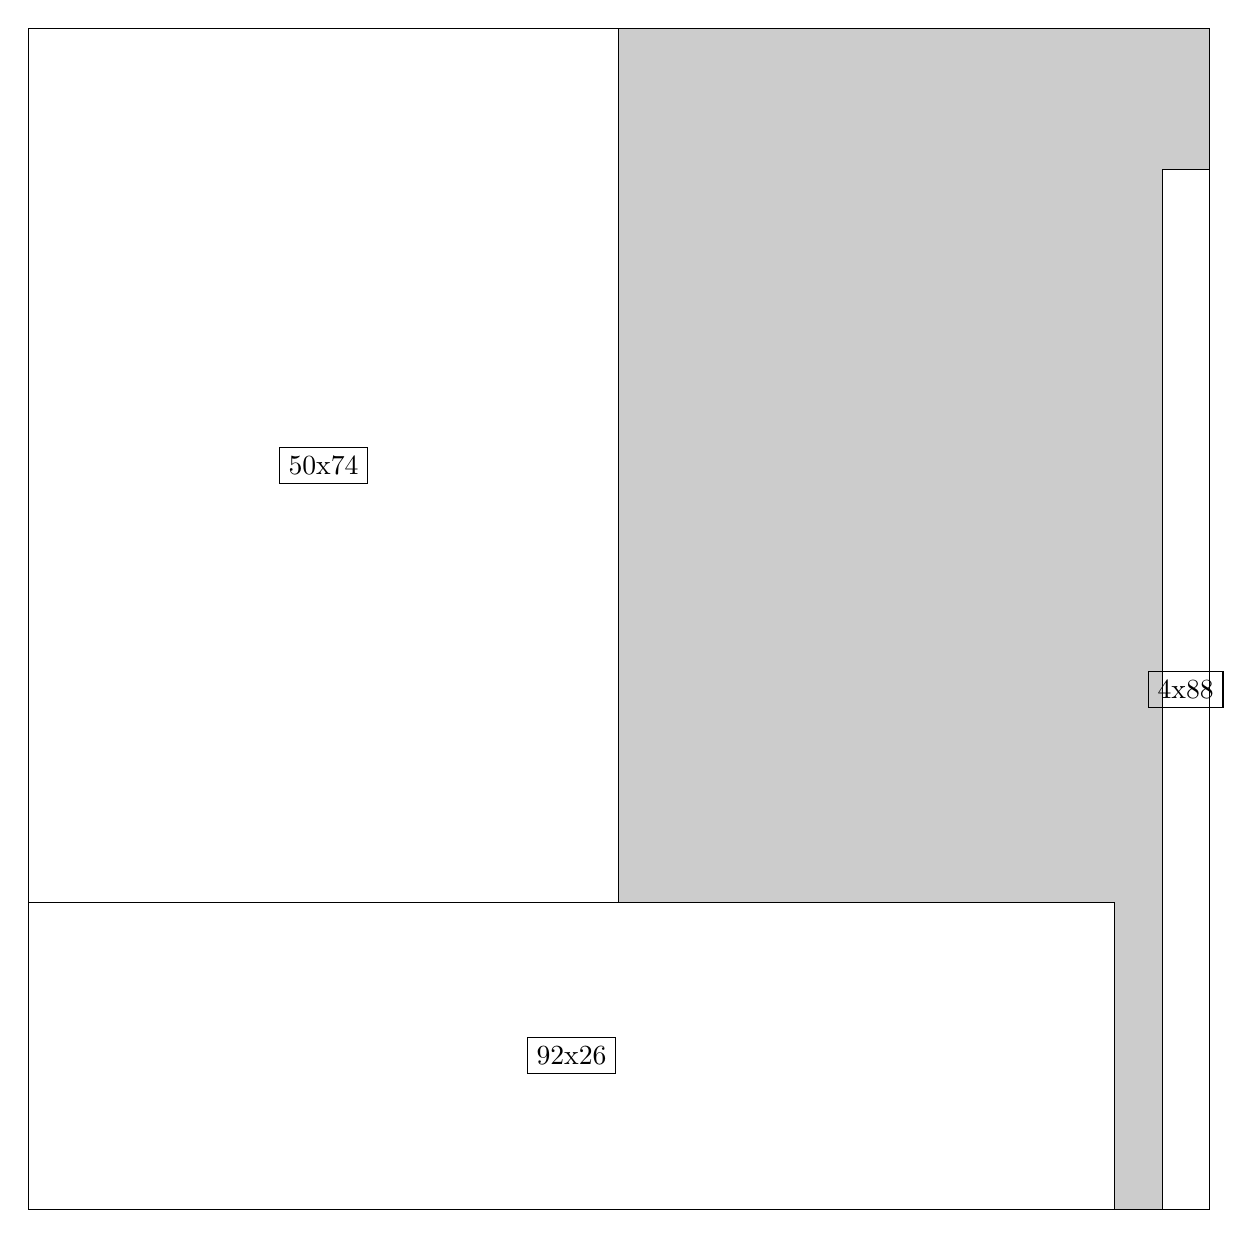
\begin{tikzpicture}[shorten >=1pt,scale=1.0,every node/.style={scale=1.0},->]
\tikzstyle{vertex}=[circle,fill=black!25,minimum size=14pt,inner sep=0pt]
\filldraw[fill=gray!40!white, draw=black] (0,0) rectangle (15.0,15.0);
\foreach \name/\x/\y/\w/\h in {92x26/0.0/0.0/13.799999999999999/3.9,50x74/0.0/3.9/7.5/11.1,4x88/14.399999999999999/0.0/0.6/13.2}
\filldraw[fill=white!40!white, draw=black] (\x,\y) rectangle node[draw] (\name) {\name} ++(\w,\h);
\end{tikzpicture}


w =92 , h =26 , x =0 , y =0 , v =2392
\par
w =50 , h =74 , x =0 , y =26 , v =3700
\par
w =4 , h =88 , x =96 , y =0 , v =352
\par
\newpage


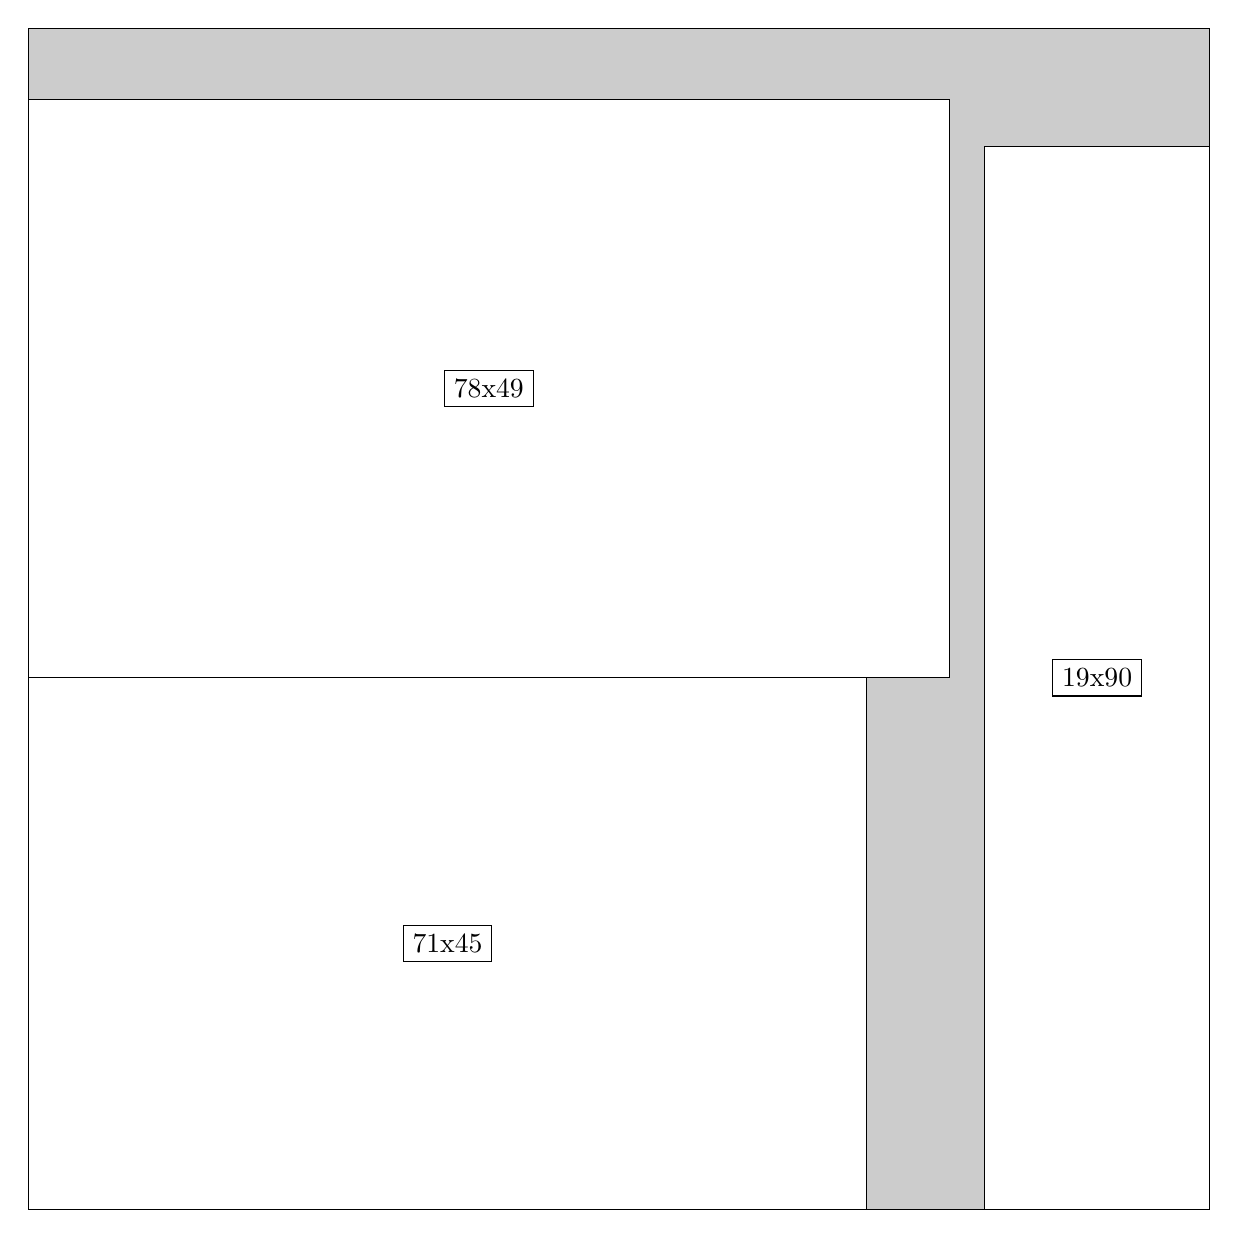
\begin{tikzpicture}[shorten >=1pt,scale=1.0,every node/.style={scale=1.0},->]
\tikzstyle{vertex}=[circle,fill=black!25,minimum size=14pt,inner sep=0pt]
\filldraw[fill=gray!40!white, draw=black] (0,0) rectangle (15.0,15.0);
\foreach \name/\x/\y/\w/\h in {71x45/0.0/0.0/10.65/6.75,78x49/0.0/6.75/11.7/7.35,19x90/12.15/0.0/2.85/13.5}
\filldraw[fill=white!40!white, draw=black] (\x,\y) rectangle node[draw] (\name) {\name} ++(\w,\h);
\end{tikzpicture}


w =71 , h =45 , x =0 , y =0 , v =3195
\par
w =78 , h =49 , x =0 , y =45 , v =3822
\par
w =19 , h =90 , x =81 , y =0 , v =1710
\par
\newpage


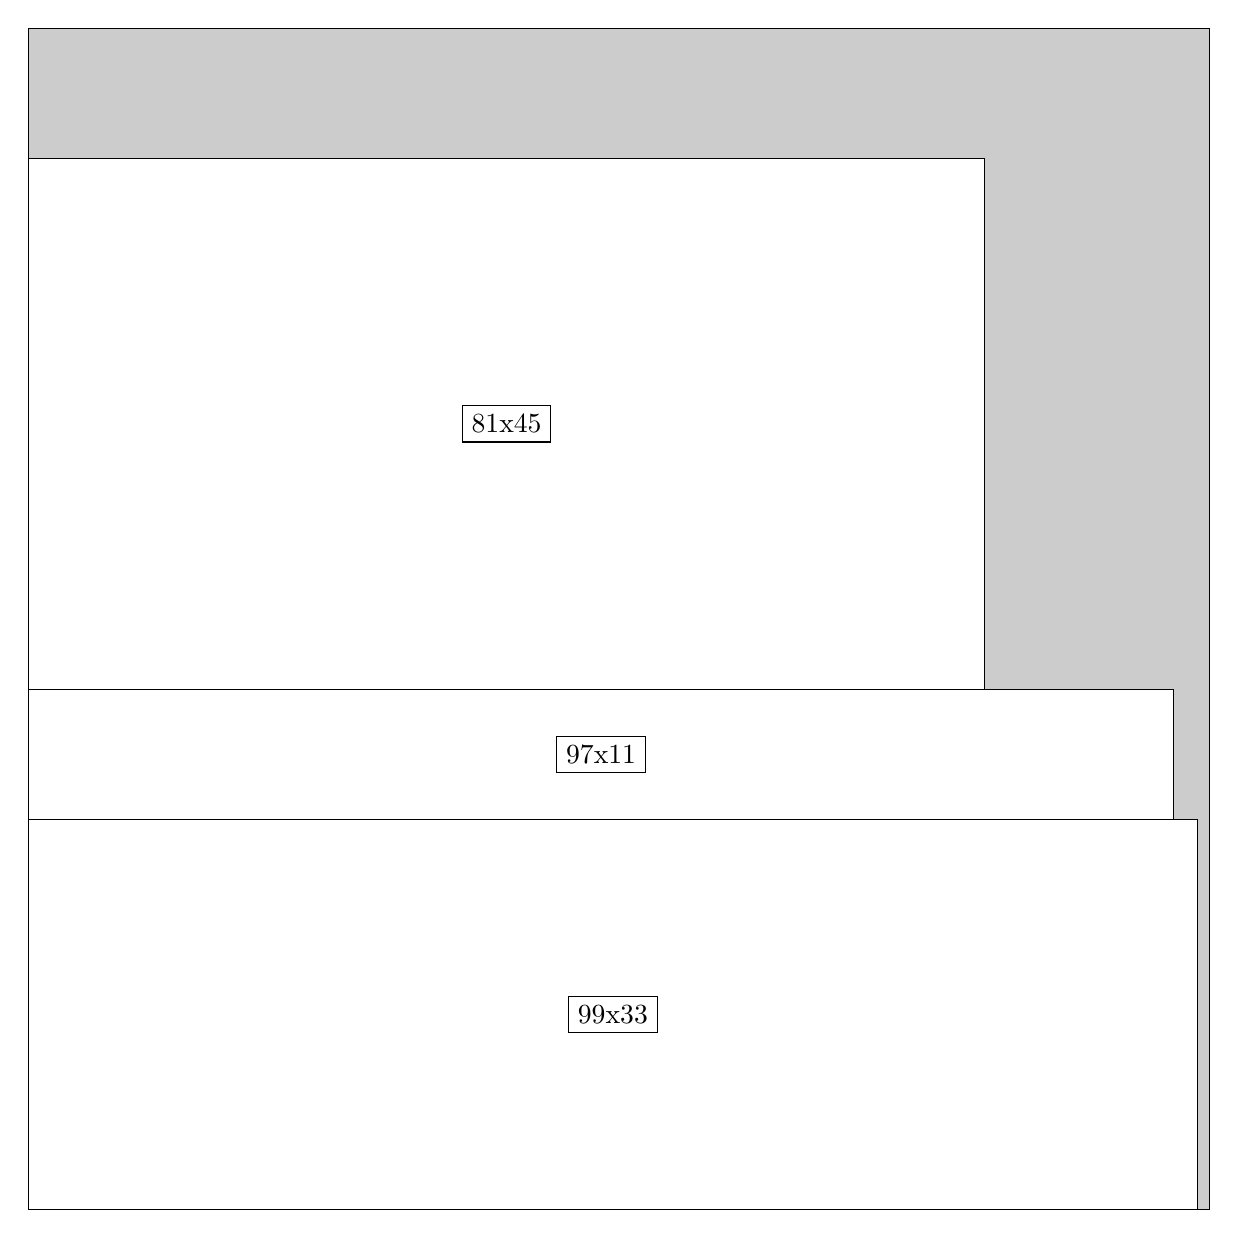
\begin{tikzpicture}[shorten >=1pt,scale=1.0,every node/.style={scale=1.0},->]
\tikzstyle{vertex}=[circle,fill=black!25,minimum size=14pt,inner sep=0pt]
\filldraw[fill=gray!40!white, draw=black] (0,0) rectangle (15.0,15.0);
\foreach \name/\x/\y/\w/\h in {81x45/0.0/6.6/12.15/6.75,99x33/0.0/0.0/14.85/4.95,97x11/0.0/4.95/14.549999999999999/1.65}
\filldraw[fill=white!40!white, draw=black] (\x,\y) rectangle node[draw] (\name) {\name} ++(\w,\h);
\end{tikzpicture}


w =81 , h =45 , x =0 , y =44 , v =3645
\par
w =99 , h =33 , x =0 , y =0 , v =3267
\par
w =97 , h =11 , x =0 , y =33 , v =1067
\par
\newpage


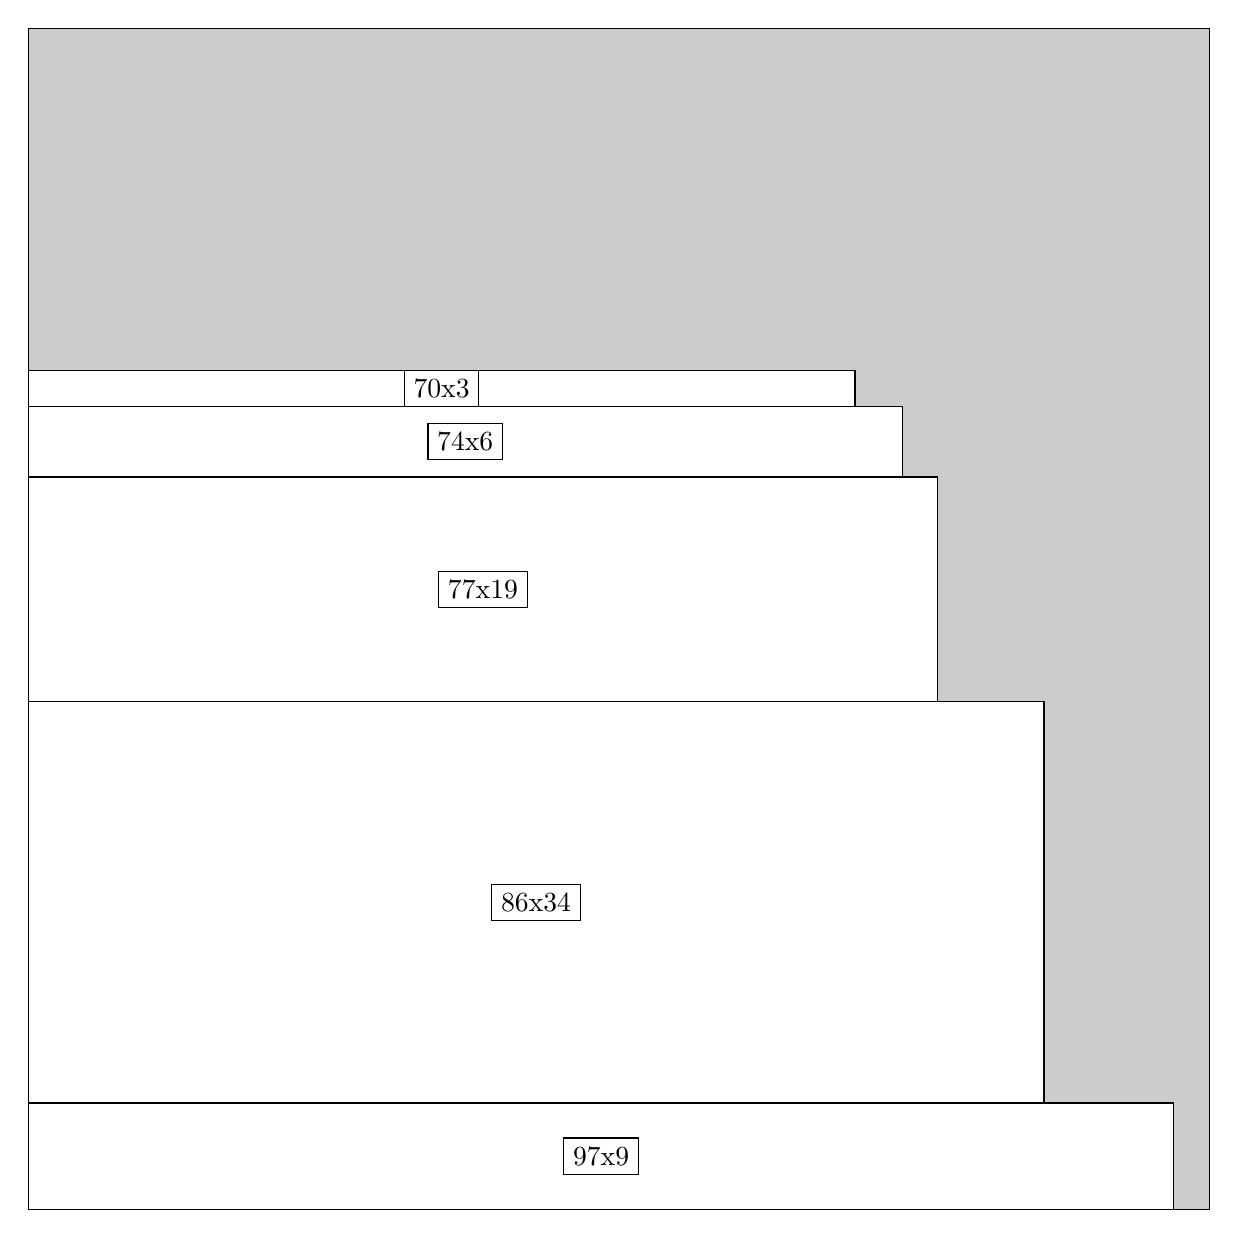
\begin{tikzpicture}[shorten >=1pt,scale=1.0,every node/.style={scale=1.0},->]
\tikzstyle{vertex}=[circle,fill=black!25,minimum size=14pt,inner sep=0pt]
\filldraw[fill=gray!40!white, draw=black] (0,0) rectangle (15.0,15.0);
\foreach \name/\x/\y/\w/\h in {86x34/0.0/1.3499999999999999/12.9/5.1,77x19/0.0/6.45/11.549999999999999/2.85,97x9/0.0/0.0/14.549999999999999/1.3499999999999999,74x6/0.0/9.299999999999999/11.1/0.8999999999999999,70x3/0.0/10.2/10.5/0.44999999999999996}
\filldraw[fill=white!40!white, draw=black] (\x,\y) rectangle node[draw] (\name) {\name} ++(\w,\h);
\end{tikzpicture}


w =86 , h =34 , x =0 , y =9 , v =2924
\par
w =77 , h =19 , x =0 , y =43 , v =1463
\par
w =97 , h =9 , x =0 , y =0 , v =873
\par
w =74 , h =6 , x =0 , y =62 , v =444
\par
w =70 , h =3 , x =0 , y =68 , v =210
\par
\newpage


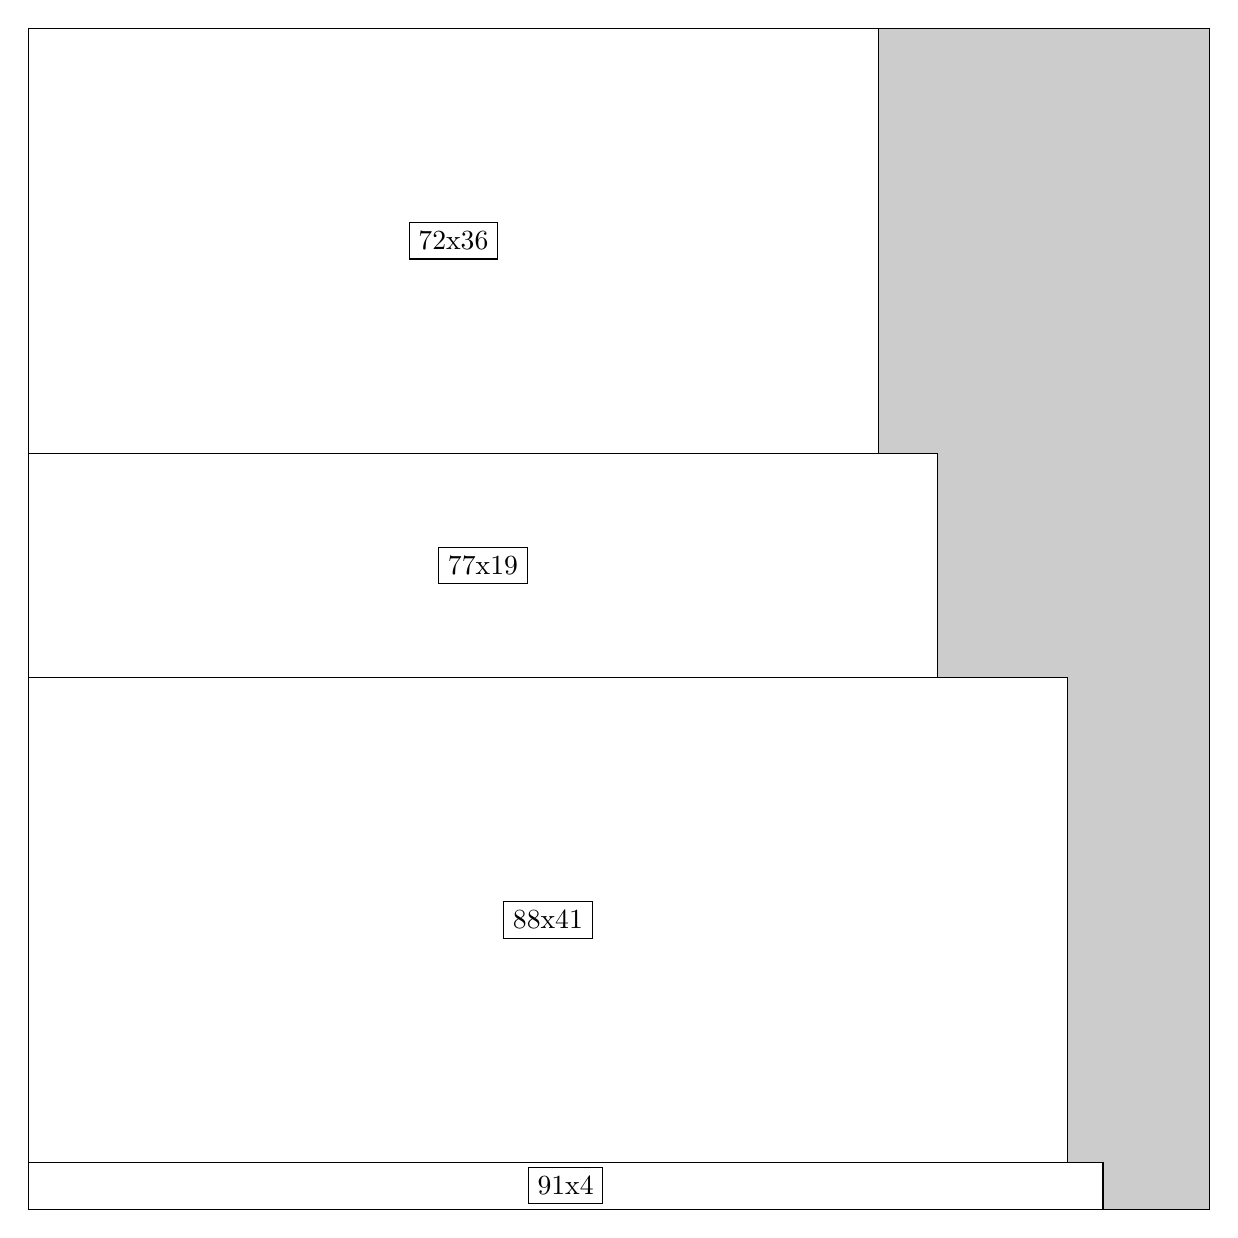
\begin{tikzpicture}[shorten >=1pt,scale=1.0,every node/.style={scale=1.0},->]
\tikzstyle{vertex}=[circle,fill=black!25,minimum size=14pt,inner sep=0pt]
\filldraw[fill=gray!40!white, draw=black] (0,0) rectangle (15.0,15.0);
\foreach \name/\x/\y/\w/\h in {88x41/0.0/0.6/13.2/6.1499999999999995,72x36/0.0/9.6/10.799999999999999/5.3999999999999995,77x19/0.0/6.75/11.549999999999999/2.85,91x4/0.0/0.0/13.65/0.6}
\filldraw[fill=white!40!white, draw=black] (\x,\y) rectangle node[draw] (\name) {\name} ++(\w,\h);
\end{tikzpicture}


w =88 , h =41 , x =0 , y =4 , v =3608
\par
w =72 , h =36 , x =0 , y =64 , v =2592
\par
w =77 , h =19 , x =0 , y =45 , v =1463
\par
w =91 , h =4 , x =0 , y =0 , v =364
\par
\newpage


\end{document}